\documentclass[12pt,a4paper]{article}

%% Language and font encodings
\usepackage[english]{babel}
\usepackage[utf8x]{inputenc}
\usepackage[T1]{fontenc}

%% Sets page size and margins
\usepackage[a4paper,top=3cm,bottom=2cm,left=3cm,right=3cm,marginparwidth=1.75cm]{geometry}
%% Useful packages
\usepackage{amsmath}
\usepackage{graphicx}
\usepackage[colorinlistoftodos]{todonotes}
\usepackage[colorlinks=true, allcolors=blue]{hyperref}
\title{Construction of 2D Orthographic Projection Views from 3D Figure and vice versa}
\author{Sushant Rathi, Shashwat Shivam}

% \documentclass{article}
\usepackage{titlesec}
\usepackage{hyperref}

\titleclass{\subsubsubsection}{straight}[\subsection]

\newcounter{subsubsubsection}[subsubsection]
\renewcommand\thesubsubsubsection{\thesubsubsection.\arabic{subsubsubsection}}
\renewcommand\theparagraph{\thesubsubsubsection.\arabic{paragraph}} % optional; useful if paragraphs are to be numbered

\titleformat{\subsubsubsection}
  {\normalfont\normalsize\bfseries}{\thesubsubsubsection}{1em}{}
\titlespacing*{\subsubsubsection}
{0pt}{3.25ex plus 1ex minus .2ex}{1.5ex plus .2ex}

\makeatletter
\renewcommand\paragraph{\@startsection{paragraph}{5}{\z@}%
  {3.25ex \@plus1ex \@minus.2ex}%
  {-1em}%
  {\normalfont\normalsize\bfseries}}
\renewcommand\subparagraph{\@startsection{subparagraph}{6}{\parindent}%
  {3.25ex \@plus1ex \@minus .2ex}%
  {-1em}%
  {\normalfont\normalsize\bfseries}}
\def\toclevel@subsubsubsection{4}
\def\toclevel@paragraph{5}
\def\toclevel@paragraph{6}
\def\l@subsubsubsection{\@dottedtocline{4}{7em}{4em}}
\def\l@paragraph{\@dottedtocline{5}{10em}{5em}}
\def\l@subparagraph{\@dottedtocline{6}{14em}{6em}}
\makeatother

\setcounter{secnumdepth}{4}
\setcounter{tocdepth}{4}
\usepackage{amsthm}
\newtheorem{definition}{Definition}


\begin{document}
\maketitle

\begin{abstract}
This paper deals with the mathematics involved in converting 3D Figures to their orthographic projections and also the methods of reconstruction of 3D figures using the given orthographic views.
\end{abstract}

\tableofcontents

\newpage

% \section{Input-Output Format}

% The input-output is assumed to be a text file with the following fields (All parameters separated by commas and different shapes/geometries are on separate lines) :-

% \begin{itemize}
%   \item Point - 'p',X1,Y1,Z1 (Co-ordinates of point)
%   \item Lines - 'l',point1,point2 (Using Previous Definition of point).
%   \item Circles - 'c',center point,radius
%   \item Circular Arc - 'a',point1,point2,point3 (These are co-ordinates of 3 points on the arc).
%   \item Ellipse - 'e',center,end1,end2 (Co-ordinates of center and ends of 2 axes in corresponding order).
%   \item Elliptical Arc - 'ea',end point1,end point2,internal point1,internal point2,internal point3
%   \item Connecting 2D Surfaces - 'conn',Surface 1 Data,Surface 2 Data
% \end{itemize}

\section{Converting 3D Figure to 2D views}

We will be converting 3D figures to 2D views by taking orthographic projections of the constituent points of the figure, and using properties of an affine transformation to connect those points. Let us first understand what the relevant terms mean.
\\ \\
\subsection{Orthographic Projections}

Orthographic projections are a a form of parallel projection in which the projection lines are orthogonal to the
projection plane, resulting in every plane appearing as an \textbf{affine transformation} on the viewing surface. (Refer to fig) One useful property of such transformations is that it preserves straight lines, which means that an edge  in a 3D projection will be a line segment connecting the projections of its end points after the transformation (unless the points are overlapping). Since we are considering polyhedral solids which can be represented by their constituent edges, being able to project vertices is all we will need to obtain the 2D views.  \newline
% \\ \\
% To determine whether a line is occluded by a face or not (for hidden lines), we need a method to check when an edge/ a portion of edge is occluded by a face.
%  \newline


\begin{figure}
\centering
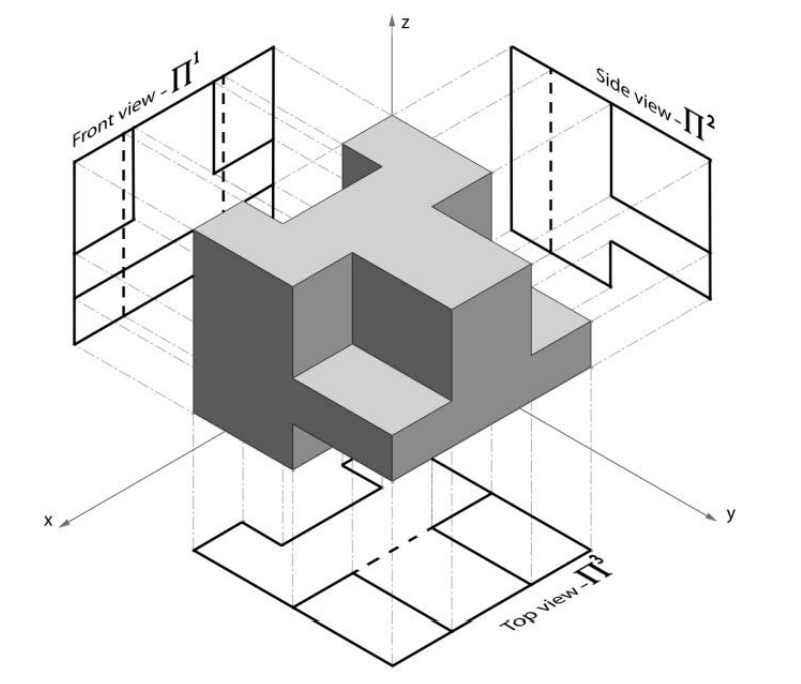
\includegraphics[width=0.3\textwidth]{Orthographic_simple.png}
\caption{\label{fig:simpleortho}Taking Projections onto different planes.}
\end{figure}



\subsection{Representation of 3D object in Input}
We assume the object description is given in terms of the 3D coordinates of the constituent points, and the edge relations (as a wireframe model). While this information is enough for obtaining 2D projections, to obtain {\textbf{hidden lines}} we will need information regarding which points constitute a face as well. We are assuming that the wireframe representation is enough to determine faces, using our algorithm described in the  section 4.3 .


\section{Straight Lines}

Considering the 2 end points of an edge, the projection can be easily taking using a projection matrix. Multiplying both the end points by projection matrices for the specific plane , we can obtain projections onto the 3 planes. \newline

Considering $ P_{xy}$ , $P_{yz}$ and $P_{xz} $ to be the projection matrices onto the respective planes and \boldmath$A$ to be the point to be projected the calculations are as follows :- 


\begin{equation}
P_{xy}  A =
\begin{bmatrix}
1&0&0\\
0&1&0\\
\end{bmatrix}
\begin{bmatrix}
X_i\\
Y_i\\
Z_i\\
\end{bmatrix}
=
\begin{bmatrix}
x_i\\
y_i\\
\end{bmatrix}
\end{equation}

\begin{equation}
P_{yz}  A =
\begin{bmatrix}
0&1&0\\
0&0&1\\
\end{bmatrix}
\begin{bmatrix}
X_i\\
Y_i\\
Z_i\\
\end{bmatrix}
=
\begin{bmatrix}
y_i\\
z_i\\
\end{bmatrix}
\end{equation}

\begin{equation}
P_{xz}  A =
\begin{bmatrix}
1&0&0\\
0&0&1\\
\end{bmatrix}
\begin{bmatrix}
X_i\\
Y_i\\
Z_i\\
\end{bmatrix}
=
\begin{bmatrix}
x_i\\
z_i\\
\end{bmatrix}
\end{equation}

Projections can also be taken onto any general plane by using a projection matrix \boldmath$P$ corresponding to that plane :- 

\begin{equation}
P  A = A'
\end{equation}

After taking the projections the points are connected by a straight line. 


\subsection{Obtaining Hidden Lines}

Hidden lines, represented as dotted lines traditionally, are lines that have been occluded in a view by other faces. To determine if a line is hidden or not, we need a method to determine whether a particular face occludes a particular edge or not, and if so what portion of it. We propose the following method for this purpose-
If the end points of an edge are enclosed inside the face projection (which will be a polygon), consider only those points for comparison.
If an end point of an edge is not enclosed , instead of the end point consider the corresponding  point of intersection (Refer to figure) .
Now that we have two representative points of the edge (say A and B), our task is to check if these two points lie on the opposite side of the face plane (opposite to the projection plane). To do so, we take any point on the face and consider its projection on the projection plane, call it X. We will now check if A and X are on opposite sides of the face plane or not. Since the edge is not intersecting the  face, all points on line segment AB lie on the same side of the plane, and hence we can say that if A and X are on opposite sides, the line segment AB is occluded 
 \newline


%
To determine if two points A and X are on same side of plane or not, we plug in the coordinates of the points in the LHS of equation of plane \(ax + by + cz - d = 0\) and compare signs- the points lie on opposite sides iff the signs are different. 
For every edge, we iterate over all faces to determine the length of segment occluded, and take a union over all lengths. 
\\ \\ \\ \\ \\
% \subsection{Circles and Ellipses}

% Projections of circles/ellipses can be circles,ellipses or straight lines with length equal to diameter. Since ellipses can be uniquely represented by using 5 points , taking any random 5 points on the circle/ellipse will give us the required set f points to regenerate the projection of the circle/ellipse onto any plane. After taking any 5 points the procedure which was used for lines is repeated to take projections. \newline

% If the Projections lie in a straight line , then the projection of the center of the circle/ellipse is taken. \newline

% After taking the projections the points are joined by an ellipse passing through the 5 points if they are not co-linear , else they are connected by a straight line and the length of the straight line is set to be equal to the radius on either side of from the center point. \newline

\begin{figure}
\centering
\includegraphics[width=0.3\textwidth]{HiddenLine.png}
\end{figure}

\section{Rotation of 3D Figures}

Rotation of 3D Figures can be interpreted easily as a multiplication of each point by a rotation matrix. After this the 2D views can be regenerated by simply projecting the new points onto the respective planes. Considering \boldmath$R$ to be the rotation matrix and \boldmath$A$ to be the point the new point will now be :- 

\begin{equation}
R  A = R'
\end{equation}

The projections can also be taken directly from the original co-ordinate system along with the rotation matrix like this :-
\begin{equation}
R P A = A'
\end{equation}

\subsection{Basic Rotation}

A basic rotation is the rotation about one of the axes of the co-ordinate system. Assuming the rotation is of an angle of $ \theta $ about the x , y and z axis respectively then the resultant co-ordinates of the rotation are as follows :-

\begin{equation}
R_{x}(\theta) A =
\begin{bmatrix}
1&0&0\\
0&\cos \theta&- \sin \theta \\
0&\sin \theta& \cos \theta \\
\end{bmatrix}
\begin{bmatrix}
X_i\\
Y_i\\
Z_i\\
\end{bmatrix}
=
\begin{bmatrix}
x_i\\
y_i\\
z_i\\
\end{bmatrix}
= A'_x
\end{equation}

\begin{equation}
R_{y}(\theta) A =
\begin{bmatrix}
\cos \theta&0& \sin \theta \\
0&1&0\\
-\sin \theta&0& \cos \theta \\
\end{bmatrix}
\begin{bmatrix}
X_i\\
Y_i\\
Z_i\\
\end{bmatrix}
=
\begin{bmatrix}
x_i\\
y_i\\
z_i\\
\end{bmatrix}
= A'_y
\end{equation}

\begin{equation}
R_{z}(\theta) A =
\begin{bmatrix}
\cos \theta&- \sin \theta&0 \\
\sin \theta& \cos \theta&0 \\
0&0&1 \\

\end{bmatrix}
\begin{bmatrix}
X_i\\
Y_i\\
Z_i\\
\end{bmatrix}
=
\begin{bmatrix}
x_i\\
y_i\\
z_i\\
\end{bmatrix}
= A'_z
\end{equation}

Here $R_x(\theta)$ ,$R_y(\theta)$ and $R_z(\theta)$ are the rotation matrices about the respective axes.

\subsection{General Rotation}

Any other general rotation can be obtained using the above three rotations . This can be done in a stepwise
manner about the three axes. The final rotation matrix $R$ is obtained as follows :-

\begin{equation}
    R= R_z(\alpha)R_y(\beta)R_x(\gamma)
\end{equation}

where $\alpha$ , $\beta$ and $\gamma$ represent the yaw , pitch and roll respectively of the rotation.

\section{Creating 3D Solids using 2D Projections}

Our method for reconstruction can be split into two parts :-
\begin{enumerate}
    \item Constructing a wire-frame model out of the given projections.
    \item Obtaining faces out of this wire-frame to define the 3D solid.
\end{enumerate}
% \textbf{Step 1} : 
% \textbf{Step 2}: 


\subsection{Assumptions}

To perform these steps in an efficient and  correct manner, we have placed the following restrictions on the input provided :
\begin{enumerate}
    \item  \textbf{We will be dealing with polyhedral solids, and hence only planar surfaces}  \hfill \\
This is mainly because we do not have a general method for reconstructing/representing quadratic surfaces. We could however extend our method to simpler objects like cylinders later on.
        \item  \textbf{The input projections will consist of labelled vertices} \hfill \\
This is because otherwise the wire-frame model obtained after step 1 can contain many pseudo elements, in the sense some of the edges/vertices may not exist in the actual solid (Refer Figure \ref{fig:ortho} and \ref{fig:solid}). Hence the algorithm for face reconstruction does not guarantee correctness- it mainly requires using some heuristics like  ensuring at least one edge from certain sets exist in the final solid, edges do not intersect faces, etc.
\end{enumerate}
\begin{figure}
\centering
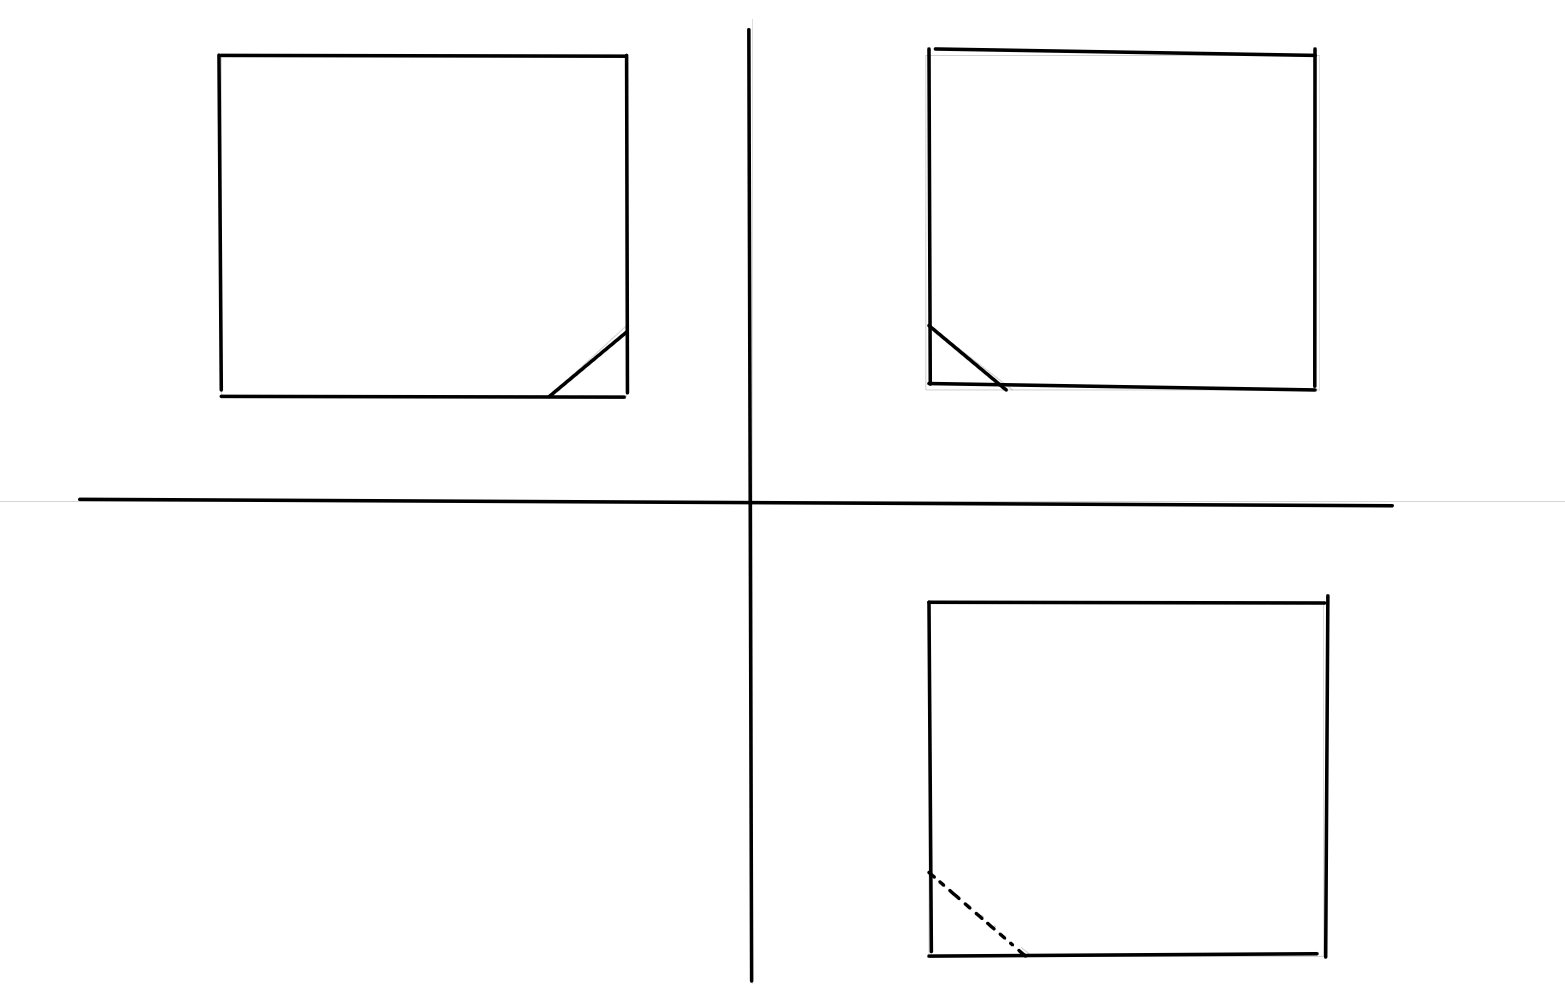
\includegraphics[width=0.3\textwidth]{Orthograph.png}
\caption{\label{fig:ortho}Given Orthographic Projections}
\end{figure}

\begin{figure}
\centering
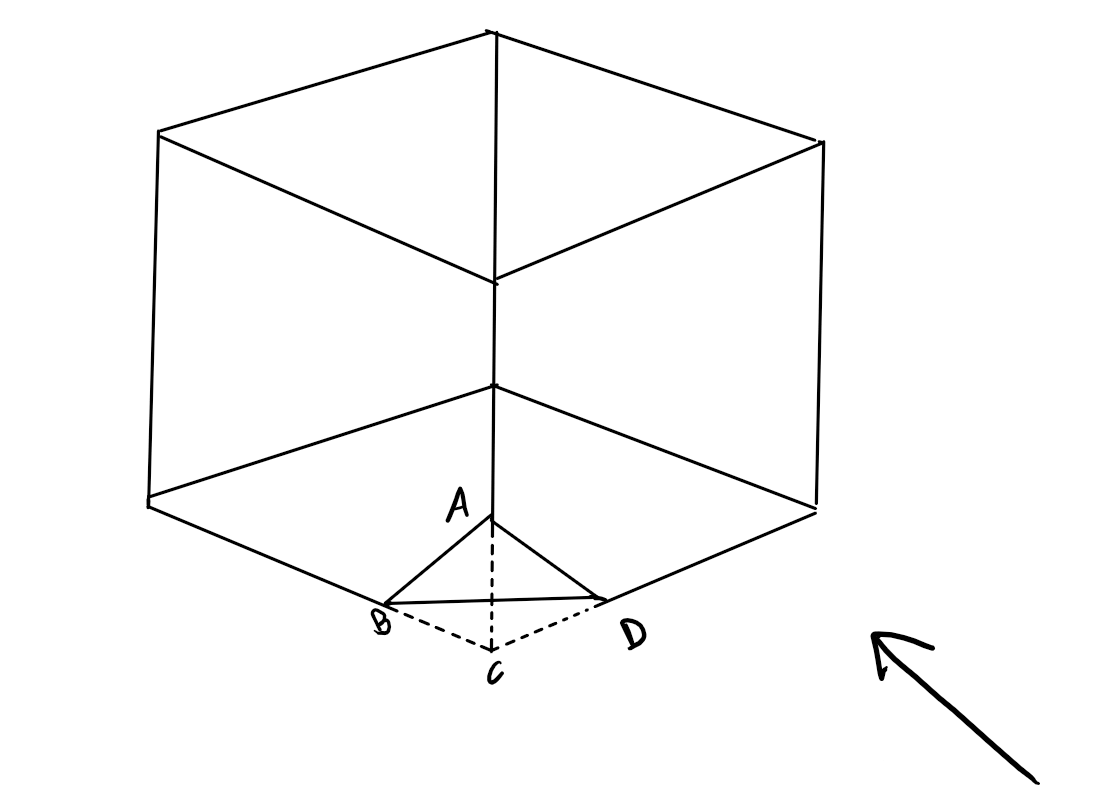
\includegraphics[width=0.3\textwidth]{Wireframe.png}
\caption{\label{fig:solid}Wireframe reconstructed can have AC,BC and CD present as well}
\end{figure}


\subsection{Step 1: Constructing a wire-frame model out of the given projections}

This process is fairly straightforward. Since every vertex is visible in every orthographic view (overlapping vertices as well), one orthographic view gives us 2 coordinates of a vertex. Hence, 2 orthographic views are sufficient to give the 3D coordinates of a vertex. To construct a wire-frame model, however, we need edge relations as well (i.e. which vertices are connected directly). Any edge in an orthographic view can be divided into two categories- either it is perpendicular to the plane of projection (in which case its projection is a point), or it is not (in which case its projection is a line segment). Thus, the existence of an edge AB implies that in each of its projections, A and B are connected either by a line segment or are overlapping, and at most one view can have overlapping points. \newline

To avoid having to check every possible pair of points for edge relations, we will pick a particular view (say top), and consider only those pair of points which have an edge connection in this particular view. We shall then check the other view for existence of line segment connecting these two points (or whether they are overlapping). \newline

Note that there is a possibility that there exist line segments in the given views between two points (say A and B) that are corresponding to different edges, that is, edges whose end-points overlap with A and B in every view. To deal this possibility, we are assuming that the input provided will indicate when there are multiple line segments overlapping in a view, in terms of relative thickness of the lines. Also, in case of overlapping points, the points will be ordered in terms of their distance from projection plane. 

\subsection{Step 2: Obtaining faces out of the wire-frame to define the 3D solid}

This algorithm, broadly speaking, consists of forming a graph with planar edge loops acting as nodes, and shared edges acting as connections between the nodes (the connection will be labeled by the name of the shared edge between the two faces). Shared edge here, as the name suggests, is an edge that belongs to both edge loops. These edge loops cannot cross each other, that is, the respective edges of any pair of edge loops can either be overlapping, or intersect at their end-points. The nodes of this graph must now be coloured as valid or invalid, with certain constraints. Before stating the constraints, let us define an edge incident set.  
\begin{definition}
An edge incident set of an edge is defined as the set of valid planar edge loops containing that edge.     
\end{definition}


Before defining what valid nodes (edge loops) are, let us recognize the fact that only looking at shared edges is not enough to determine if an area bounded by edge loops is a  face or not. This is because a portion of area of a loop can be ‘cutoff’ by another edge loop inside, due to the existence of a hole/extrusion. 

To formalize this, let us make a few definitions regarding edge loop containment. \\ \\
% \begin{itemize}
\begin{definition}
     An edge loop X is said to be contained inside another edge loop Y iff all vertices of X lie inside the area bounded by Y.  \\  \\
\end{definition}
    % \item \textbf{Def 1}:
    
    \begin{definition}
     If an edge loop X is contained in Y, and there exists no edge loop Z such that X is contained in Z and Z is contained in Y, X is said to be predecessor of Y.
        \\ 
\end{definition}
  
% \end{itemize}


Now let us define what a valid edge loop  is.
\begin{definition}
     A planar edge loop X  (graph node) is said to be valid if the region between X and all its predecessors forms a face.
\end{definition}

\begin{figure}
\centering
\includegraphics[width=0.3\textwidth]{edgeLoop.png}
\end{figure}

\begin{figure}
\centering
\includegraphics[width=0.3\textwidth]{LoopInsideLoop.png}
\end{figure}


It is easy to see that if X is valid, all its predecessors will be invalid, as both being valid would imply that the edges forming its predecessors have faces on both sides, which would make that edge redundant. Also, if X is invalid, all its predecessors will be valid, otherwise the third constraint stated will be violated.

Thus, if we construct a poset of edge loops defined on the relation of containment, we can say that for any poset S with a least element, determining the validity of any edge loop belonging to S will determine the validity of every other edge loop belonging to S. \cite[see chapter 4]{bagchi}

 Given the previous definitions, the constraints we must follow in our reconstruction  are-
\begin{enumerate}
    \item The cardinality of every edge incident set is exactly two.
    \item No two edge loops belonging to an edge incident set share the same plane.
    \item No two  edge loops not belonging to an edge incident set of an edge E, but containing E, can be planar.
\end{enumerate}



These constraints follow  from the fact that the faces form a 2-manifold without boundary. \cite{principals} \newline

Thus, the construction of edge loops will proceed as follows. 
\begin{enumerate}

    \item  We will first divide all the edges into sets of co planar edges. After this, for every set we will obtain a set of edge loops. Assuming we have edge adjacency relations (by common vertices), this can be done by simply starting at an edge and running a depth first search from it, and repeating the process for an edge not visited.
    \item Once this is done, for the set of edge loops, we construct posets defined on the containment relation as defined earlier. This poset will be useful later as determining validity of any element of a poset determines validity of every other element as well.
    \item Now for every edge E, we consider its the set of edge loops it is a part of (call it S(E) ). If the cardinality of S(E) is 2, both edge loops must be valid (this follows from first constraint). Thus, we shall first consider only those edges that satisfy this condition. (If the 2 loops are coplanar, we have violated the second constraint, and hence a 3D solid is not possible). For every edge loop X discovered as valid/invalid, we now determine the validity of edge loops of the poset which X is a part of. After every new discovery, we enforce constraints 2 and 3, which means that if two edge loops belonging to S(E) are planar, exactly one of them is valid.
    \item We repeat the process for the remaining edges, where we maintain count of the elements belonging to its edge incidence set. If we cannot find any edge for which the condition stated in 3 holds, we will have to perform branching. This means we will consider a particular edge loop to be valid, and repeat steps 3 and 4 from then onwards. 
    \item If we reach at an impossible state from this branching, we backtrack, reversing the last decision we made. We terminate the process either when we have managed to colour all the nodes (and not violated any constraint along the way), or we have looked at all possibilities but have not arrived at an admissible solution.

\end{enumerate}

% \begin{figure}
% \centering
% \includegraphics[width=0.3\textwidth]{edgeLoop.png}
% \end{figure}

% \begin{figure}
% \centering
% \includegraphics[width=0.3\textwidth]{LoopInsideLoop.png}
% \end{figure}

% 3D Solids are generated from 2D Projections using a step-wise method which involves the following steps :-
% \begin{itemize}
% \item Recovering Vertices existent in 3D Solids
% \item Recovering 2D curves 
% \item Generating Edges (True and False both)
% \item Generating Surfaces
% \item Marking Solid/Non Solid Areas and finding a solution satisfying the postulates
% \item Removing False Volumes
% \end{itemize}
% The assumed postulates are as follows :-
% \begin{itemize}
% \item 
% \end{itemize}
% \subsection{Generating 3D Vertices}
% To generate 3D vertices we look at the vertices in 2D in any one of the view. If there exists a third co-ordinate such that the generated points projections are also vertices in other 2 views then we take this point as a vertex.
% \subsection{Recovering 2D Curves}
% If any point is left in 2D which is not a projection of any vertex in 3D then it may be part of a curve. For curves we take any 2 points of the extremes and 3 points in between and find out the possible co-ordinates of points on the curve in 3D by using other views .
% \subsection{Generating Edges}
% To generate edges we look at the generated 3D vertices and check if the pair of vertices are connected in all of the view by a line. If they are we connect the vertices by an edge in 3D too.
% \subsection{Generating Surfaces}

% \section{Introduction}

% Your introduction goes here! Some examples of commonly used commands and features are listed below, to help you get started. If you have a question, please use the help menu (``?'') on the top bar to search for help or ask us a question. 

% \section{Some examples to get started}

% \subsection{How to include Figures}

% First you have to upload the image file from your computer using the upload link the project menu. Then use the includegraphics command to include it in your document. Use the figure environment and the caption command to add a number and a caption to your figure. See the code for Figure \ref{fig:frog} in this section for an example.

% % \begin{figure}
% % \centering
% % \includegraphics[width=0.3\textwidth]{frog.jpg}
% % \caption{\label{fig:frog}This frog was uploaded via the project menu.}
% % \end{figure}

% \subsection{How to add Comments}

% Comments can be added to your project by clicking on the comment icon in the toolbar above. % * <john.hammersley@gmail.com> 2016-07-03T09:54:16.211Z:
% %
% % Here's an example comment!
% %
% To reply to a comment, simply click the reply button in the lower right corner of the comment, and you can close them when you're done.

% Comments can also be added to the margins of the compiled PDF using the todo command\todo{Here's a comment in the margin!}, as shown in the example on the right. You can also add inline comments:

% \todo[inline, color=green!40]{This is an inline comment.}

% \subsection{How to add Tables}

% Use the table and tabular commands for basic tables --- see Table~\ref{tab:widgets}, for example. 

% \begin{table}
% \centering
% \begin{tabular}{l|r}
% Item & Quantity \\\hline
% Widgets & 42 \\
% Gadgets & 13
% \end{tabular}
% \caption{\label{tab:widgets}An example table.}
% \end{table}

% \subsection{How to write Mathematics}

% \LaTeX{} is great at typesetting mathematics. Let $X_1, X_2, \ldots, X_n$ be a sequence of independent and identically distributed random variables with $\text{E}[X_i] = \mu$ and $\text{Var}[X_i] = \sigma^2 < \infty$, and let
% \[S_n = \frac{X_1 + X_2 + \cdots + X_n}{n}
%       = \frac{1}{n}\sum_{i}^{n} X_i\]
% denote their mean. Then as $n$ approaches infinity, the random variables $\sqrt{n}(S_n - \mu)$ converge in distribution to a normal $\mathcal{N}(0, \sigma^2)$.


% \subsection{How to create Sections and Subsections}

% Use section and subsections to organize your document. Simply use the section and subsection buttons in the toolbar to create them, and we'll handle all the formatting and numbering automatically.

% \subsection{How to add Lists}

% You can make lists with automatic numbering \dots

% \begin{enumerate}
% \item Like this,
% \item and like this.
% \end{enumerate}
% \dots or bullet points \dots
% \begin{itemize}
% \item Like this,
% \item and like this.
% \end{itemize}

% \subsection{How to add Citations and a References List}

% You can upload a \verb|.bib| file containing your BibTeX entries, created with JabRef; or import your \href{https://www.overleaf.com/blog/184}{Mendeley}, CiteULike or Zotero library as a \verb|.bib| file. You can then cite entries from it, like this: \cite{greenwade93}. Just remember to specify a bibliography style, as well as the filename of the \verb|.bib|.

% You can find a \href{https://www.overleaf.com/help/97-how-to-include-a-bibliography-using-bibtex}{video tutorial here} to learn more about BibTeX.

% We hope you find Overleaf useful, and please let us know if you have any feedback using the help menu above --- or use the contact form at \url{https://www.overleaf.com/contact}!

\bibliographystyle{alpha}
\bibliography{sample}

\end{document}